%%% Copy to Setup.tex, break at the point software is needed. %%%
\index{spool holder}
\index{filament arm}
\index{filament spool}
\index{spool}
\glossary{Spool}{Plastic Filament coiled and stored on a plastic reel. Preferred due to improved feeding and better mounting options.}
\glossary{Filament}{Plastic material in "string" like form, as is fed to the printer.}
\glossary{ABS}{Acrylonitrile Butadiene Styrene thermoplastic. Usually extrudes at 230C.}
\glossary{PLA}{Polylactic Acid is a corn-based biodegradable polymer. Usually extrudes at 185C.}
\glossary{HDPE}{High Density Polyethylene.}
\glossary{Polycarbonate}{A strong and impact resistant thermoplastic. Usually extrudes at ~300C.}
\glossary{HIPS}{High Impact Polystyrene.}
\glossary{Laywoo-D3}{Wooden filament similar to PLA. Contains 40 percent recycled wood. Usually prints at ~180C- 210C. Color can be changed by varying the extrusion temperature.}

Before you start printing you will need to load a reel of filamant onto the filament arm. The filament arm is meant to work with 1kg and 5lb plastic filament reels but can be modified to work with other reel and spool types. 

\begin{enumerate}

\item On the front right hand side of the TAZ 2.1 3D printer you will find the filament arm (fig. \ref{fig:filament_arm}, page \pageref{fig:filament_arm}). Place the filament reel on the filament arm with the filament feeding counter clockwise.

\begin{figure}[H]
\centering
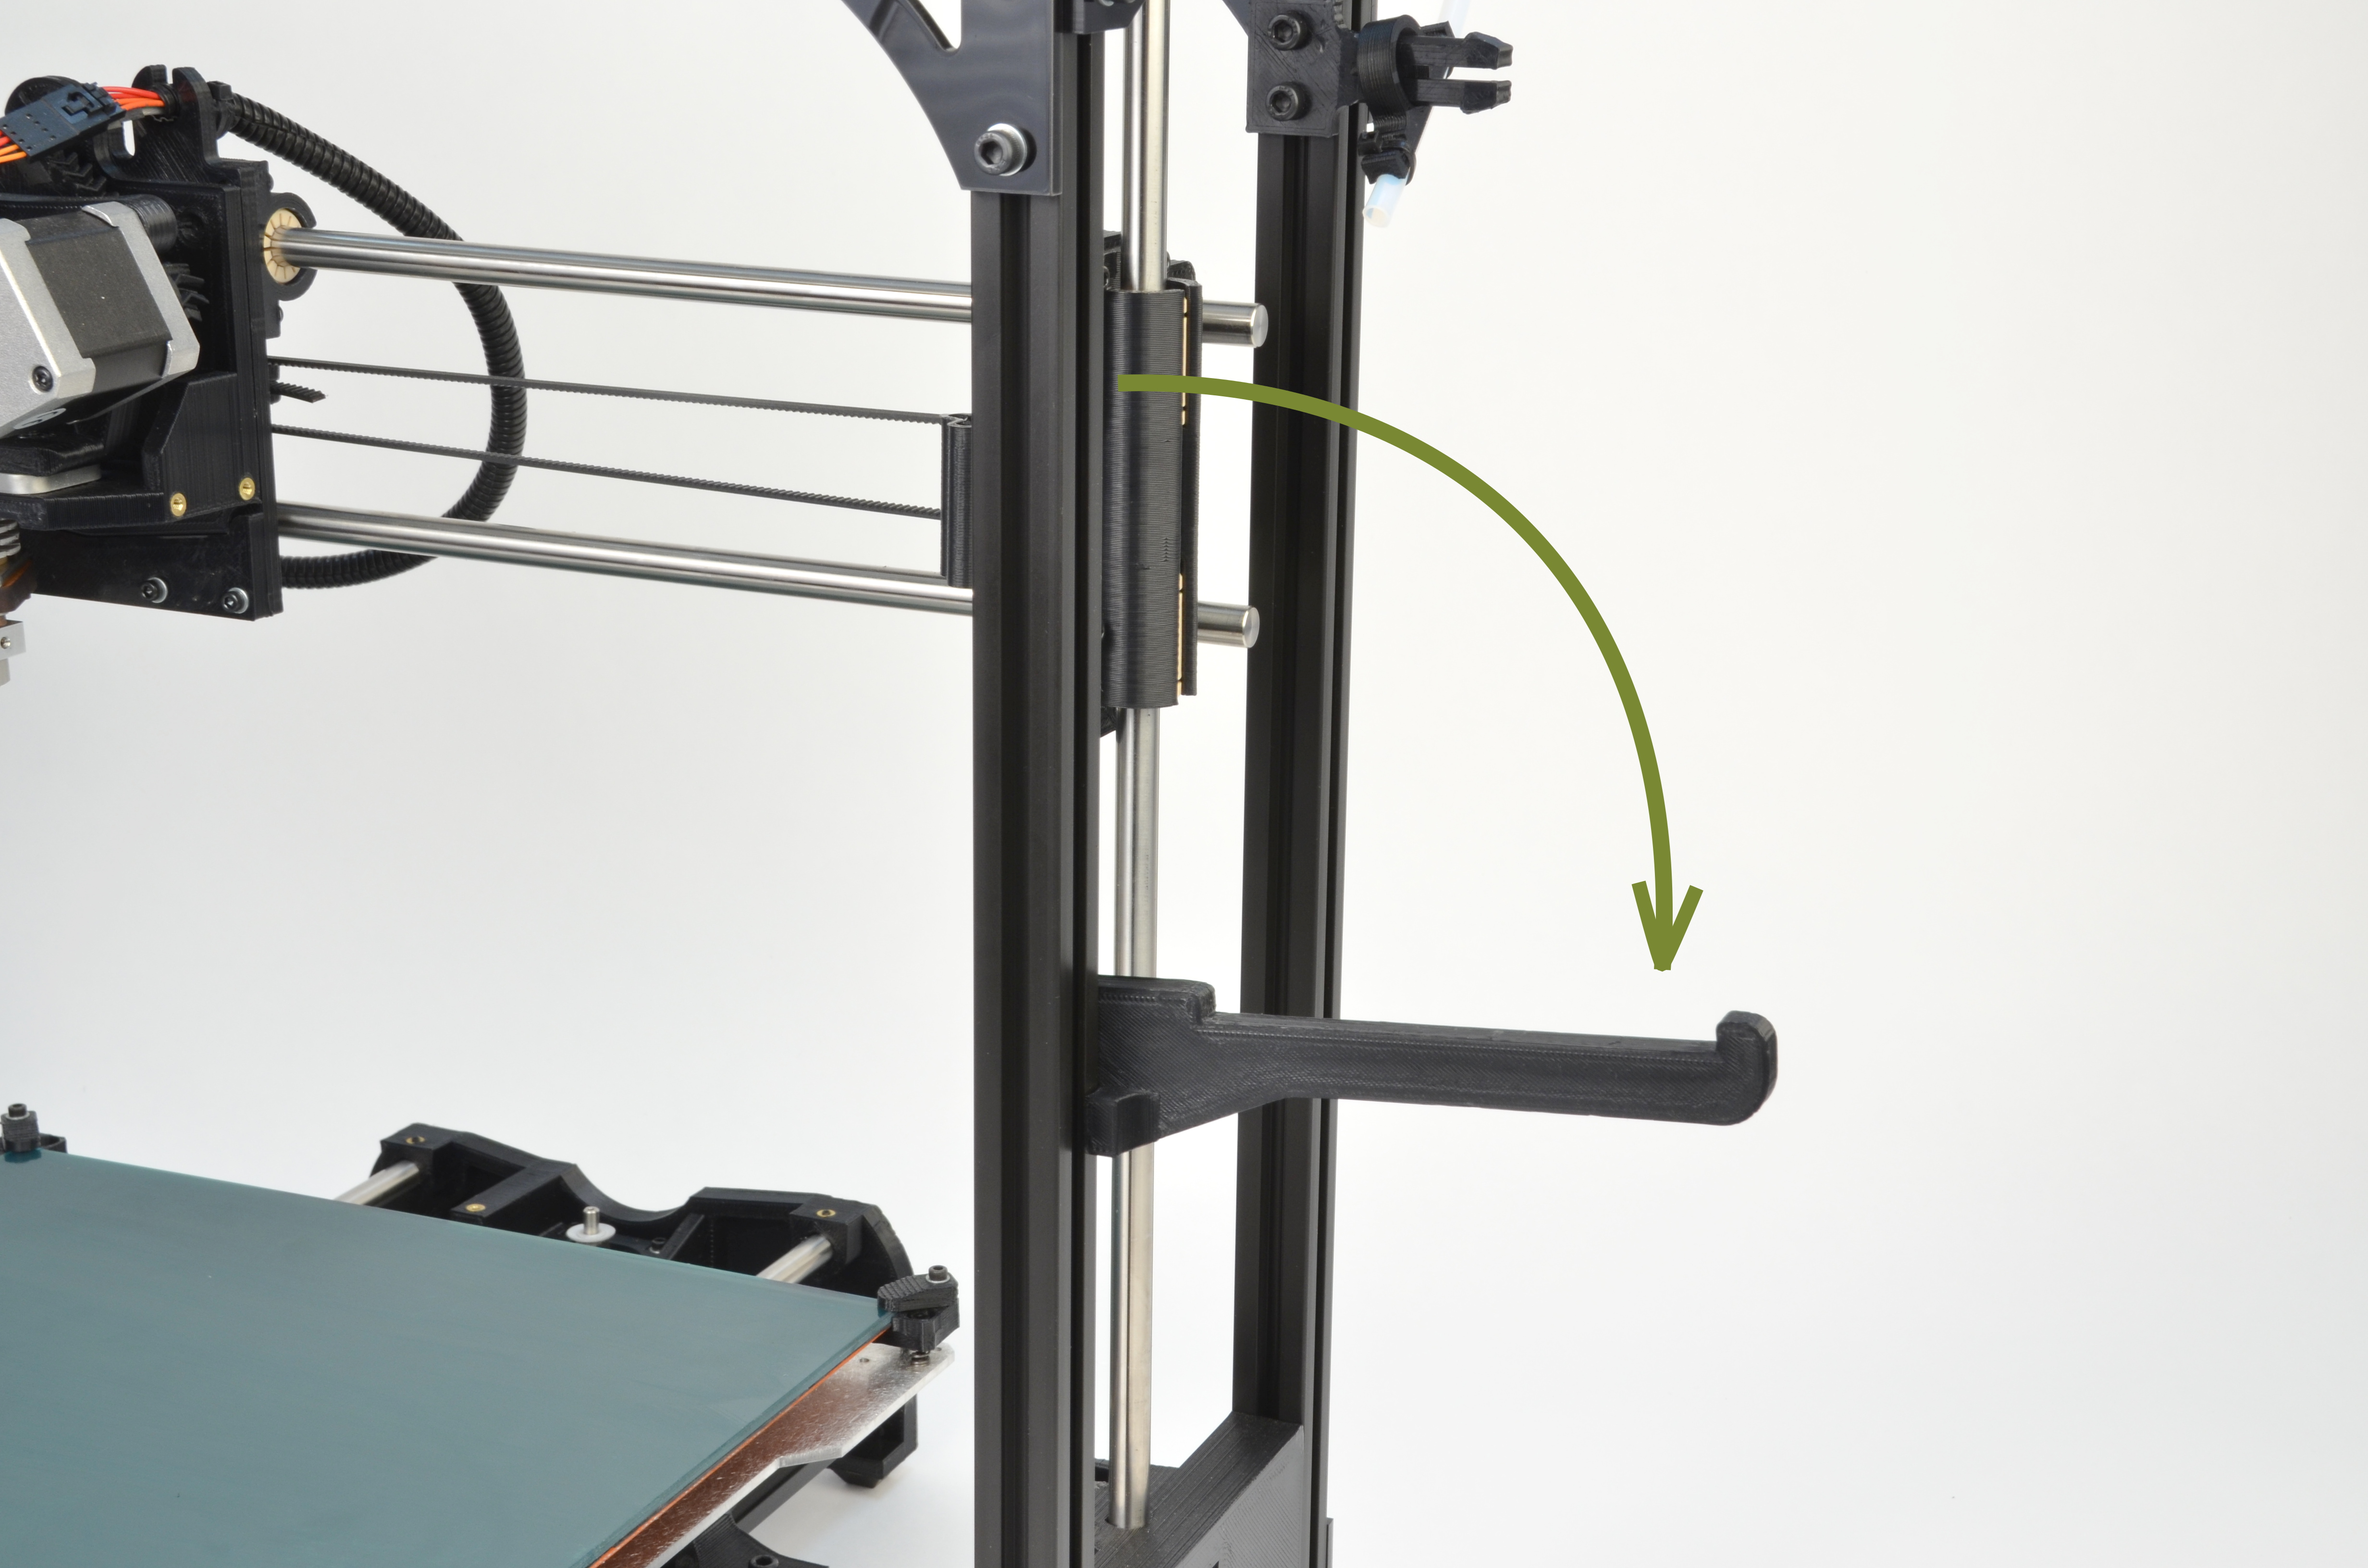
\includegraphics[keepaspectratio=true,angle=0,height=0.4\textheight,width=1.0\textwidth]{filament_arm.JPG}
\caption{Filament reel arm}
\label{fig:filament_arm}
\end{figure}

\index{feed tube}
\item Feed the end of the filament through the filament feed tube. The Filament should now be threaded through the PTFE sleeve and exiting near the extruder (fig. \ref{fig:filament_arm_loaded}, page \pageref{fig:filament_arm_loaded}).

\begin{figure}[H]
\centering
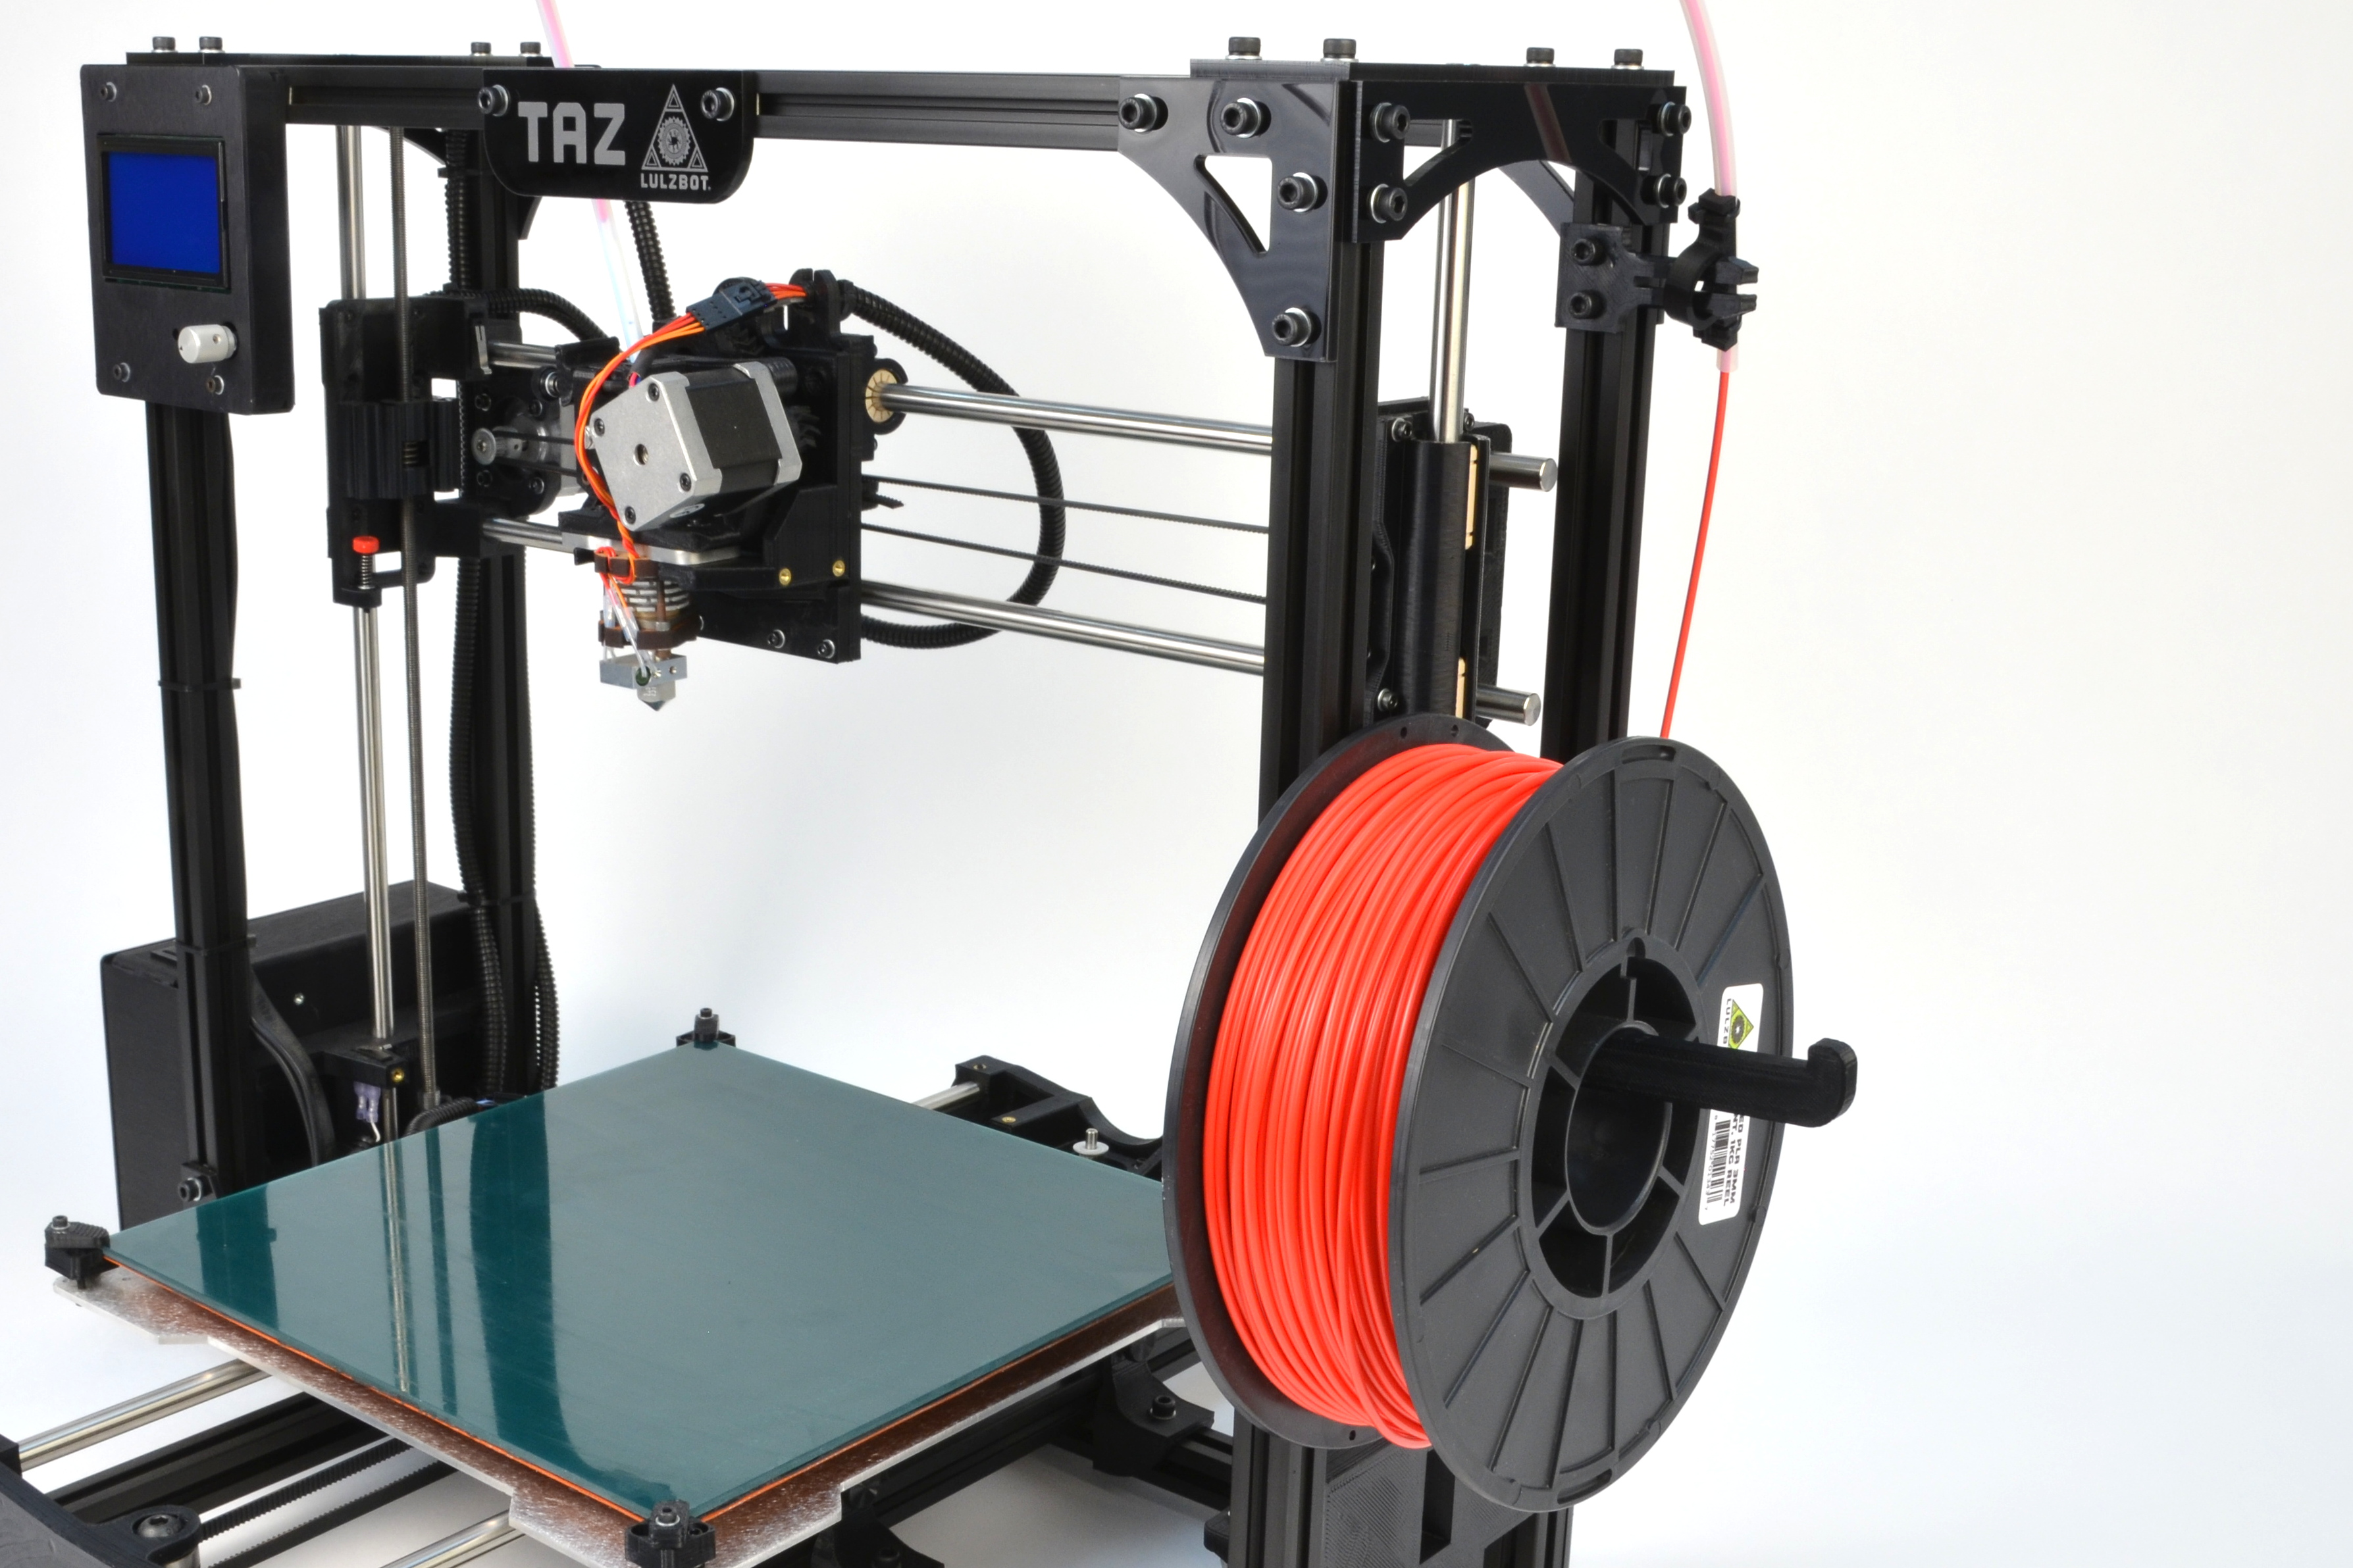
\includegraphics[keepaspectratio=true,angle=0,height=0.4\textheight,width=1.0\textwidth]{filament_arm_loaded.JPG}
\caption{Filament run through the guide}
\label{fig:filament_arm_loaded}
\end{figure}

\item Your filament reel is now mounted and ready for the next steps.

\item When changing filament, slide the opposite end of the filament through one of the holes in hub of the filament spool. This will keep the filament from unwinding from the spool.

\end{enumerate}

